\newcommand{\Msun}{\ensuremath{\mathrm{M}_\odot}}

On 14th September 2015, both the LIGO detectors recorded a GW signal consistent with what GR would predict when two BHs with masses $\sim 36 \Msun$ and $29 \Msun$ inspiraled and merged \cite{gw150914detection}. For reporting the statistical confidence of this detection, the data from a total coincident observation time of $16$ days \footnote{after applying the data quality vetoes}  was used for the analysis. From this data, a noise background equivalent to 608000 years was produced by performing unphysical time delays. The statistic used by the LIGO collaboration for detection is an empirically re-weighted combined SNR details of which can be found in \cite{detectionStat1}. On analysing the data containing GW150914 event, it was found that this event has a combined SNR of 23.6 and a false alarm probability of $\sim 2 \times 10^{-7}$. The statistical significance of this event was reported to be 5.1 $\sigma$. 

GW150914 was an extraordinarily loud event. It could be visually seen after performing just some basic filtering on the raw detector data. In section \ref{sec:dirrect-comparision}, we present a direct comparison of the raw data from the detectors (with minimal non-aggressive filtering) overlayed with a GR predicted BBH template \footnote{The models of GWs that are used in matched filtered searches are calleed as templates.}. The template corresponds to a BBH system with parameters reported by the search pipeline. In this study we see that there is a visual consistency between the observed data and the best-fit template reported by the seach pipeline. 

Although the search pipeline reports a rough estimate of the BBH parameters, a careful Bayesian parameter estimation needs to be carried to extract the astrophysical parameters of the system. In section \ref{sec:prop-GW150914}, we summarize the astrophysical parameters of GW150914 inferred by the LIGO collaboration. This section attempts to highlight a few points from \cite{gw150914PE} and \cite{gw150914PEseobnrv3}.  

\section{Direct comparison of the data and best fit template}
\label{sec:dirrect-comparision}
In this section, we describe a priliminary analysis done soon after the detection of GW150914. The basic premise of this work was to check for visual consistency between the observed signal and the best-fit template reported by the search pipeline. A more refined version of this study was performed by the LIGO collaboration and is presented as Figure 1 of \cite{gw150914detection}. 

\subsection{Filtering the data}
The raw GW strain seen by the LIGO detectors are recorded in a channel called GDS-CALIB-STRAIN. The data in this channel is calibrated but no other data quality vetoes are applied. We use the timeseries recorded in this channel and perform a minimal set of filtering needed to visually see the GW event. We first whiten the data (i.e) apply inverse detector power spectral density (PSD) curve. Then, the data is band passed and the harmonics of power-line frequencies are notched out using an analytical zero-pole-gain(zpk) filter. The filter is depicted in the bottom right inlay panel of figure \ref{fig:overlayGW150914}. The filter amplitude is set to 1 at 100 Hz. The data is filtered forward and backward to ensure that filtering does not introduce a phase error. Further, the filter is acausal (specifically, symmetric in time) and is designed to introduce zero-phase offset. This can be seen in the top right inlay panel of figure \ref{fig:overlayGW150914}. 

\subsection{Best-fit template parameters}
The search pipeline used to detect CBC signals is based on matched filtering the detector data against the expected GW templates. A template bank is created and for each template in this bank, a match filtered operation is carried out. The parameters of the tempate that maximizes match is reported by the pipeline as the best fit parameter. 

Below, we enlist the parameters of the best-fit template reported by the search pipeline PyCBC obtained by analyzing the streach of data containing GW150914. We use these parameters both for  generating andthe for  aligning the best-fit template on the raw data from the detector to produce figure \ref{fig:overlayGW150914}. 

\begin{itemize}
\item m1=47.9 $\Msun$
\item m2=36.6 $\Msun$
\item s1=0.96
\item  s2=-0.89
\item Effective distance
	\begin{itemize}
	\item L1: 1194.9118 Mpc 
	\item H1: 970.70534 Mpc
	\end{itemize}
    
\item Template phase
	\begin{itemize}
	\item L1: 0.58 radians
	\item H1: -2.77 radians
	\end{itemize}
\item Ringdown parameters
	\begin{itemize}
	\item f=228Hz
	\item Q=3.651
	\end{itemize}

\end{itemize}

\subsection{Aligning the data and the template}

The search pipeline reports the peak of the SNR time series as the merger time. Note that this time may vary slightly when the search is performed using the different template families (also known as waveform approximants) and depends on the convention of defining the $t_{merger}$ in the waveform family. In order to overlay the best-fit template on to the detector data time series, one would need a time-domain template with appropriate parameters. However, typically the search uses a frequency domain template in order to increase computational efficiency. For this study, we construct a template bank consisting of a single time-domain template corresponding to the parameter described above (i.e) the best-fit parameter reported by the search. We then perform a search on the data containing the event using this single-template template bank and record the reported time of the merger. This reported time of merger is used to align the raw data from the two detectors. Furthermore, it is also used to align the best-fit template to the data to produce the overlay plot presented in figure \ref{fig:overlayGW150914}. The merger times we obtain in our study are listed below. 

\begin{itemize}
\item L1: 1126259462.415039062 sec
\item H1: 1126259462.422363281 sec.  
\end{itemize}

This corresponds to a time delay of 7.32 ms between the Livingston (L1) and Hanford (H1) detector. Our analysis uses a sampling of 16384Hz and therefore, to align the data from the two detectors, we shift the raw data of H1 by 120 sample points. The data is also appropriately phase shifted to obtian alignment presented in Figure \ref{fig:overlayGW150914}.

From Figure \ref{fig:overlayGW150914} we find a visual agreement between the raw detector data and the best-fit template reported by the search pipeline. We can see that the data from the two detectors can be coherently aligned in phase with each other and also with the best-fit template. 

\begin{figure*}
\subfloat{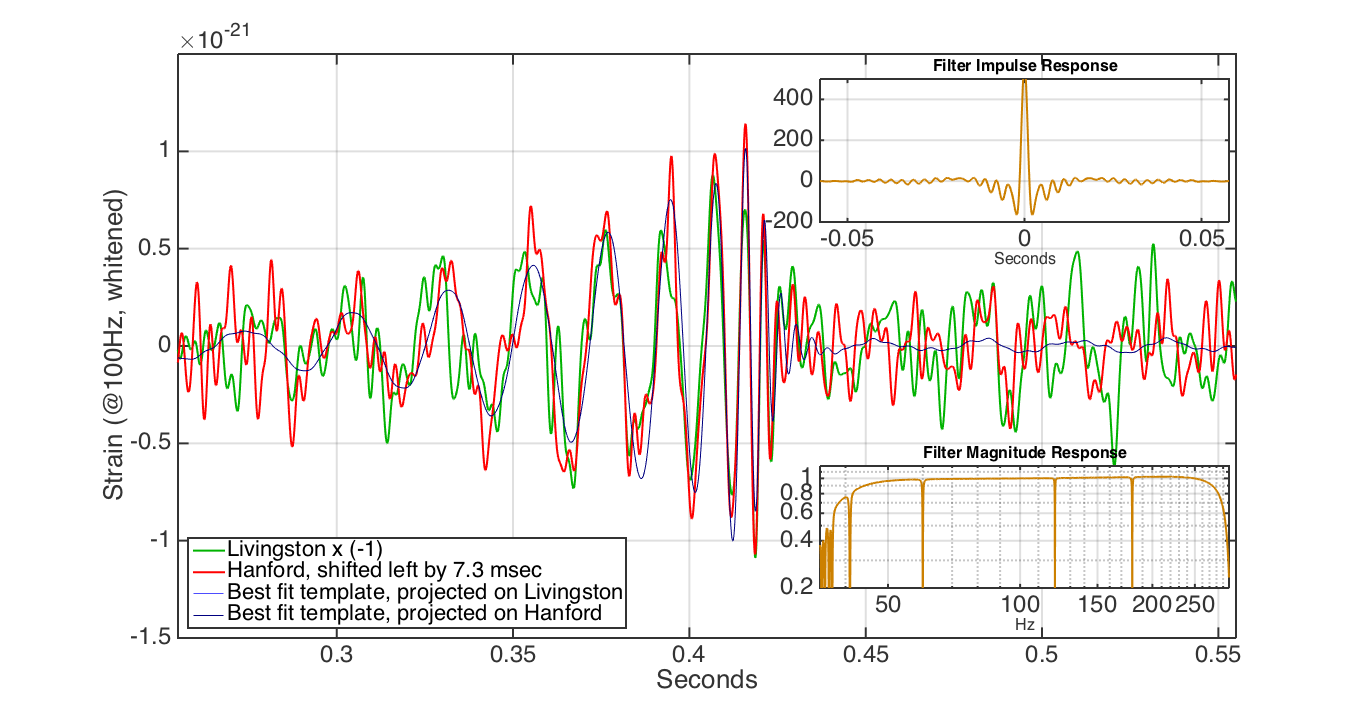
\includegraphics[width=\textwidth]{figures/overlayGW150914.png} }
\caption{Direct comparison of the detector data with the best fit template. The data from the H1 and L1 have been minimally filtered and  appropriately shifted to align with each other. The best fit template corresponding to each of the detector timeseries is overlayed on the data. The inlay panel display the details of the filters used to condition the data}
\label{fig:overlayGW150914}
\end{figure*}

\section{Properties of GW150914 using SEOBNRv3 waveforms}
\label{sec:prop-GW150914}
In the interest of computation efficiency and speed, the template banks used in the search tend to be too sparse for accurate parameter estimation of the source system.
Although the searches provide a rough estimate of the astrophysical parameters of the source system, a more careful Bayesian parameters estimation needs to be performed to extract astrophysical information from the event.   

Initially in the original PE analysis of GW150914 reported in \cite{gw150914PE}, the PE was performed using two waveform template families. The idea behind performing the PE using two different template families independently was to understand the possible effects of systematics of waveform models effecting the estimate of the parameters of the system. Below is a brief description of the two template families used to report parameters of GW150914 in \cite{gw150914PE}.
.  
\begin{enumerate}
\item SEOBNRv2 (c.f \cite{SEOBNRv2-paper} for details) is a time-domain template family that models BBH mergers using an effective one body formalism \cite{the-damour-paper}. This template family, however restricts the BHs to have spin either aligned or anti-aligned with the orbital angular momentum of the system (aligned/anti-aligned progenitor system). For computational efficiency and speed, a reduced ordered modeling of this template family in frequency domain  
called SEOBNRv2-ROM-DoubleSpin was used to perform the PE reported in\cite{gw150914PE}.

\item IMRPhenomPv2  (c.f \cite{} for details)  is an inspiral–merger–ringdown model that phenomenologically models the three phases of BBH signal. Unlike the previous, this model allows for mis-aligned spins of the BH, thereby capturing the precession physics during the insprial phase of the BBH evolution.  
\end{enumerate}

The results obtained by the two familes are very similar and we the systematic bias arising from waveform modeling does not seem to be large (c.f. Table 1 in \cite{gw150914PE} for the difference in the estimated mean values of astrophysical parameters of the system using the two waveform families listed above). Furthermore, an upgraded version of effective one body formalism was implemented which included the precession physics and the full Bayesian analysis was redone on the event data. The implementation of this called SEOBNRv3. The PE analysis preformed on the GW150914 with this new waveform family is presented in \cite{gw150914PEseobnrv3}. The two precessing models agree very well with each other, and the systematic bias in the estimated parameter was seen to reduce even more. Furthermore, it is seen that including the precession effect in the waveform modeling improves the estimate of BH spins. The results of PE as well as effect of systematics due to waveform model is beautifully visualized in Figure 1 of \cite{gw150914PEseobnrv3}, which for the convenience of the readers is presented below in Figure \ref{fig:GW150914-PE-plot}.

\begin{figure*}
\subfloat{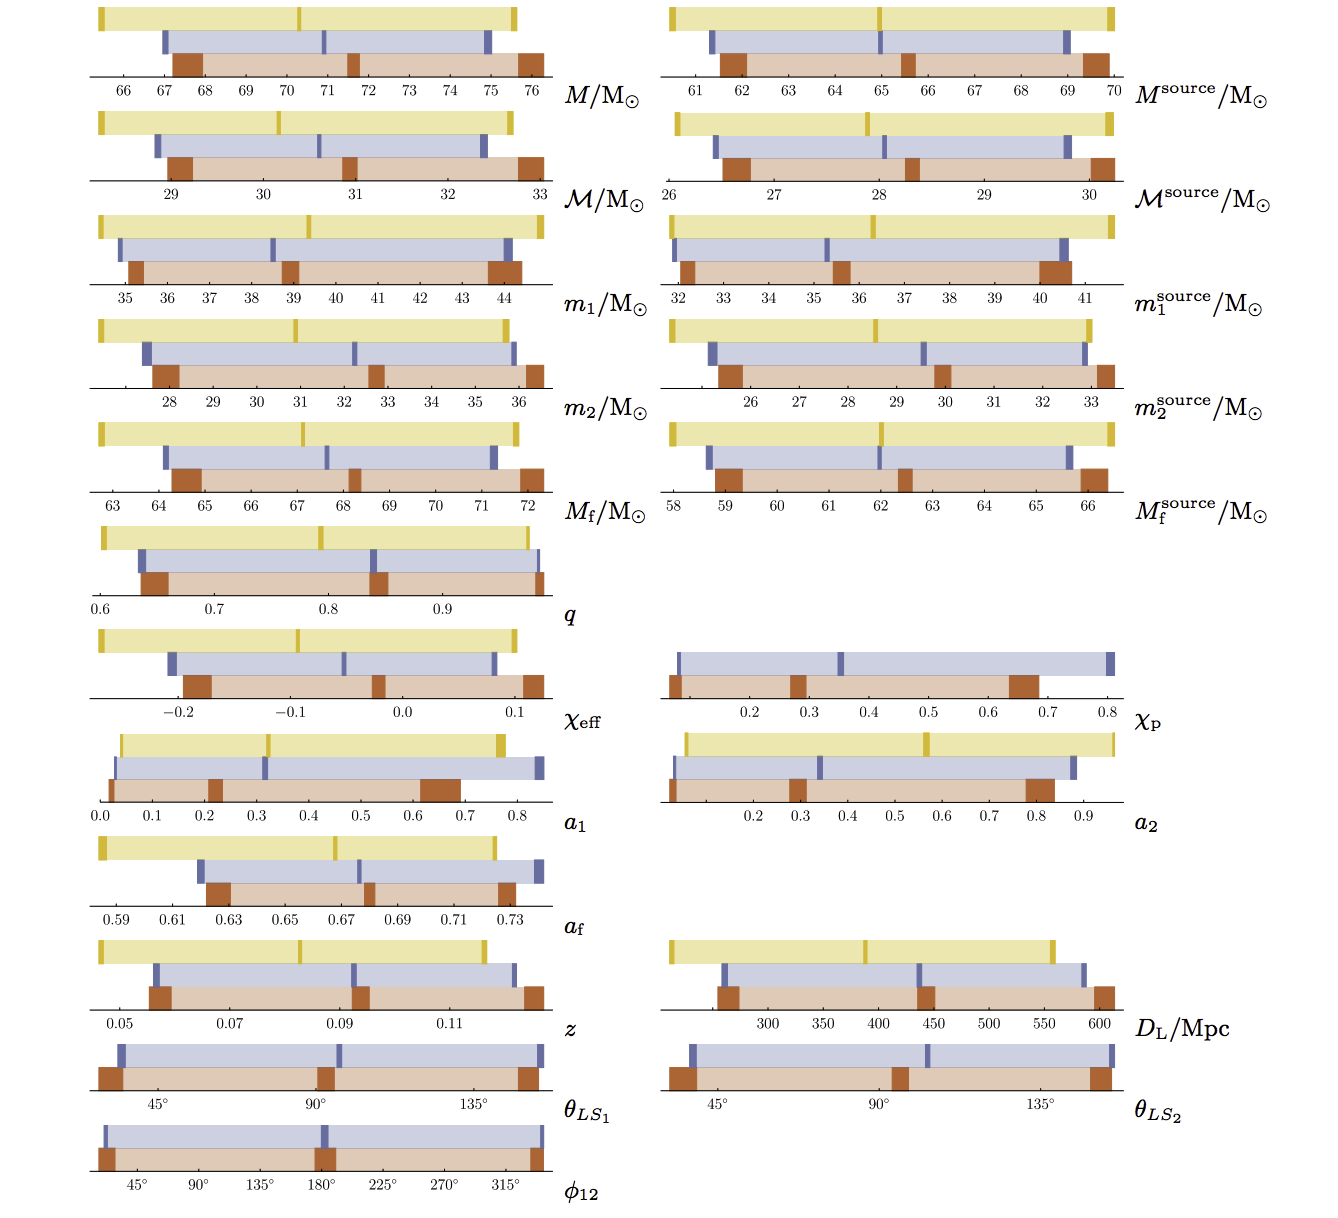
\includegraphics[width=\textwidth]{figures/PEGW150914.png} }
\caption{Astrophysical properties of GW150914. This figure presents the astrophysical parameters inferred from data corresponding to the event GW150914. The yellow bar shows the PE results obtained using non-precessing EOBNR model SEOBNRv2-ROM-DoubleSpin, blue bar corresponds to that obtained using precessing phenomenological model IMRPhenomPv2. The red bar at the bottom corresponds to the precessing EOB model. 90\% credible intervals are presented with the darker interval marking 5\%, 50\% and 95\% quantiles. Taken from \cite{gw150914PEseobnrv3}.} 
\label{fig:GW150914-PE-plot}
\end{figure*}



